
\hypertarget{working_app}{}
\section{Application options}
\index{application options}

\begin{figure}[H]
  \begin{center}
    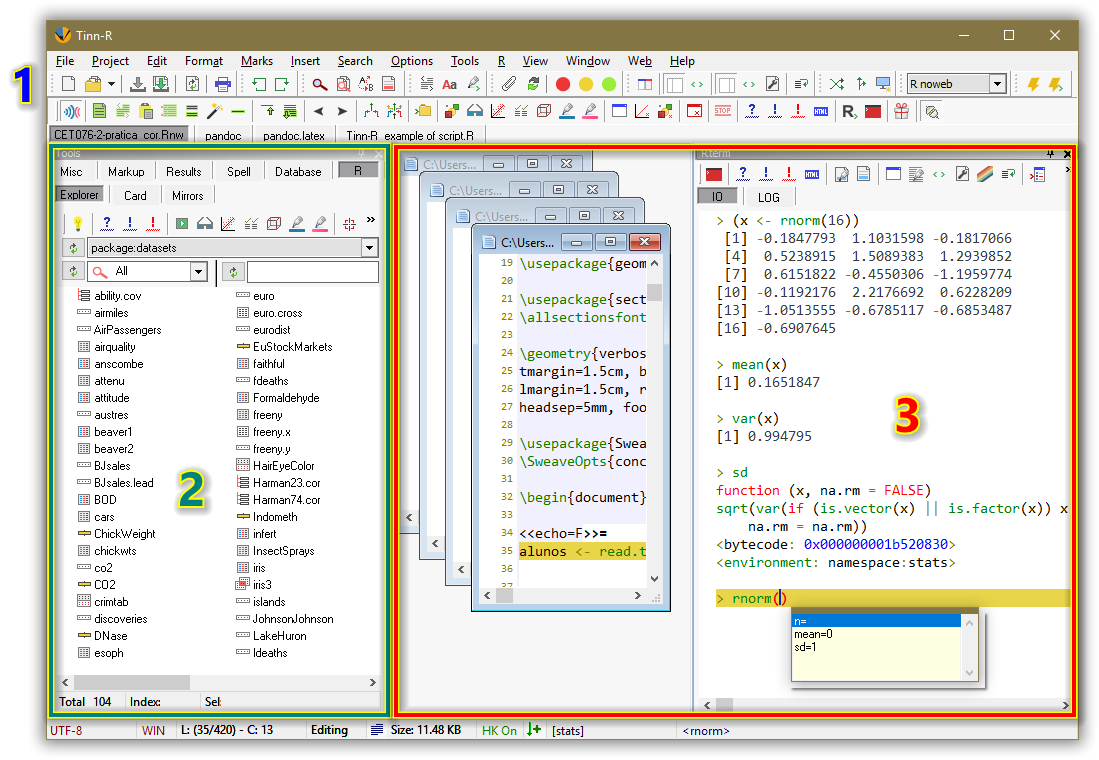
\includegraphics[width=\headwidth]{./res/parts_01.png}
  \end{center}
  \caption{Tinn-R: Main resources.}
  \label{fig:tinn-r_interface}
\end{figure}

Tinn-R interface
(Figure \ref{fig:tinn-r_interface})
is very flexible and user configurable. It is necessary time
to know all available resources and to configure this out (according to your
preferences) in a nice way. The default set of options might not be suitable
for every user.

The window \textit{Application options} allows the user to set the major piece
of user preferences related to the application.

It must be clear from now on that the Tinn-R project is the sum of three main
resources (Figure \ref{fig:tinn-r_interface}):
The application \texttt{per se (1)},
additional \texttt{Tools (2)} and
the instances of the \texttt{SynEdit class (3)}.
The \texttt{Tools (2)} was projected to allows the expansion of resources.
\index{application options}

The options visible in all pictures reflect a set of the project leader preferences.


\hypertarget{working_app_main}{}
\subsection{Main}
\index{application options!main}

\begin{figure}[H]
  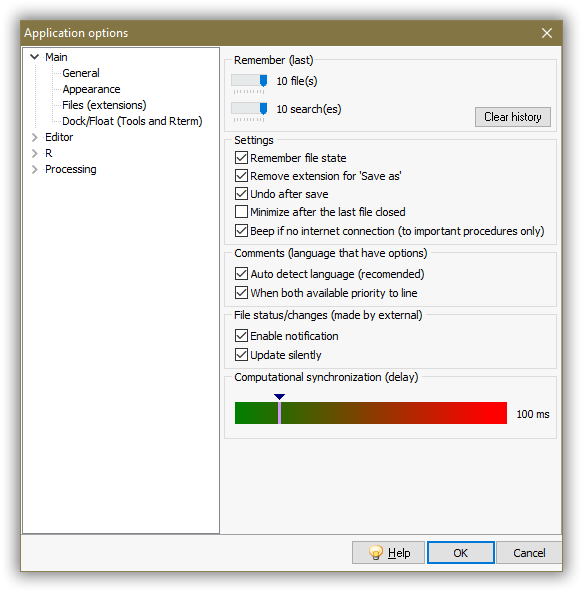
\includegraphics[scale=0.35]{./res/app_main_general.png}~~
  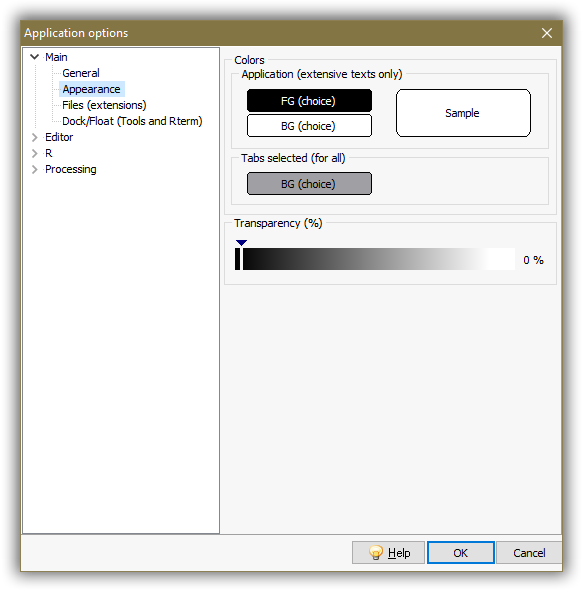
\includegraphics[scale=0.35]{./res/app_main_appearance.png}\\
  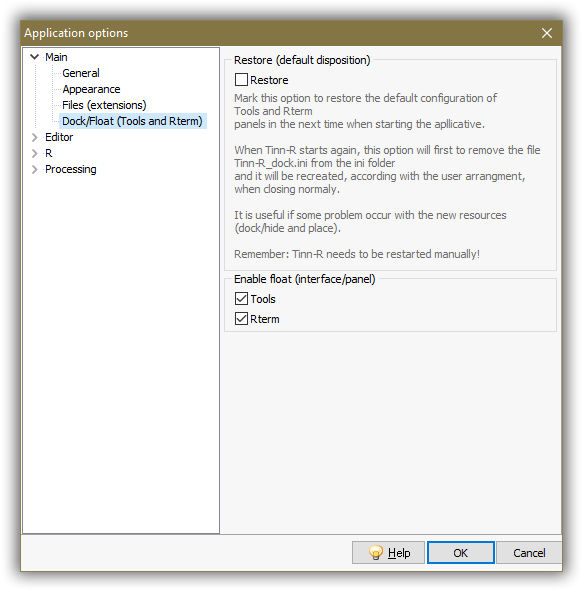
\includegraphics[scale=0.35]{./res/app_main_dock.png}~~
  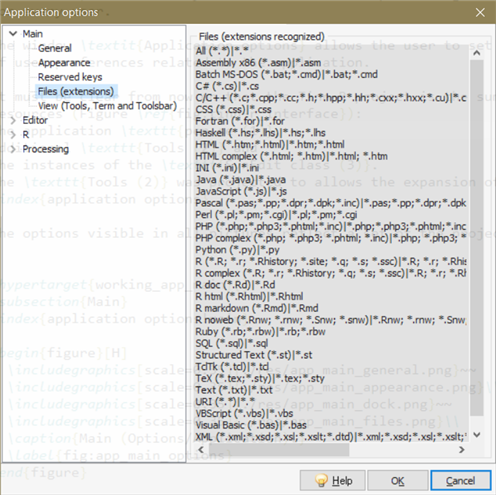
\includegraphics[scale=0.35]{./res/app_main_files.png}\\
  \caption{Main (Options/Application).}
  \label{fig:app_main_options}
\end{figure}

\begin{table}
  \begin{footnotesize}
    \begin{tabularx}{\headwidth}{>{\hsize=0.35\hsize}X>{\hsize=0.65\hsize}X}\\
      \hline
      \textbf{Option} & \textbf{Description} \\
      \hline
      Computational syncronization (delay) & Several processes are dependent on synchronization between applications
       (\RR{}, converters, compilers). The optimal value of the delay is determined by the following characteristics:
       user habits, hardware and software available.
       The ideal value is unique to the various possible combinations of those three characteristics.
       Try to reduce to the minimum value (50 ms) and test it: if something does not work, increase it gradually
       and keep testing until getting to the optimal value. The default value (100 ms) may not be optimal for all users. \\
      Remove extension for \textit{Save as} & All file extensions will be removed
       in the \textit{Save as} Windows interface \\
      Application colors (extensive text only) & Dark colors (low level of radiation)
       for the background, and pale light (high level of radiation) for the characters
       are reccomended for people who work with the computer/monitor for long periods.
       Pictures of this user guide ire like this \\
      \hline
    \end{tabularx}
  \end{footnotesize}
  \caption{Same main options}
  \label{tab:app_main}
\end{table}

Figure \ref{fig:app_main_options} and
Table \ref{tab:app_main}
show the options related to this topic.

Since the options are self-explanatory, Table \ref{tab:app_main} only gives some
details about the most difficult options to understand.


\hypertarget{working_editor}{}
\subsection{Editor}
\index{application options!editor}

The \textit{Editor} window
(Figures \ref{fig:editor_display}, \ref{fig:editor_advanced})
was adapted from the sources of the
\textit{SynEdit} component, mainly related to the general appearance and
standard options. The set of options available complement the
\textit{Application options} and allows high level of customization.


\hypertarget{working_editor_display}{}
\subsubsection{Display:}
\index{application options!!editor display}

\begin{figure}[H]
  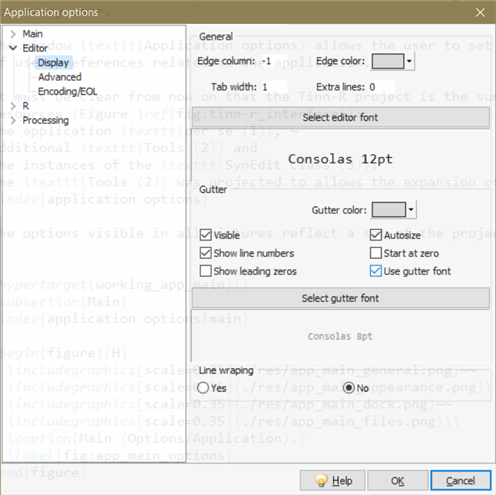
\includegraphics[scale=0.50]{./res/app_editor_display.png}~~
  \caption{Editor options: Display.}
  \label{fig:editor_display}
\end{figure}

\begin{table}
  \begin{footnotesize}
    \begin{tabularx}{\textwidth}{>{\hsize=0.3\hsize}X>{\hsize=0.7\hsize}X}\\
      \hline
      \textbf{Option} & \textbf{Description} \\
      \hline  %Display-----
      Edge column & Will be showed as a vertical line in the editor and the default is 80 characters.
      Set it to 0 or a negative value (-1) to make the edge column not visible \\
      Edge color & Choice of the edge color \\
      Tab width & Set the number of characters that will be inserted when typing the \textit{Tab} key \\
      Extra lines & Set the width which each single line will be displayed \\
      Font & Will open the Windows interface for choosing installed fonts \\
      \hline %Gutter-----
      Gutter color & Will open the Windows interface to choose a color \\
      Visible & Visibility option \\
      Autosize & Autosize option \\
      Show line number & Show line number option \\
      Start at zero & Start at zero option \\
      Show leading zeros & Show leading zeros option \\
      Use gutter font & Use gutter font option \\
      \hline
    \end{tabularx}
  \end{footnotesize}
  \caption{Display (Options/Editor).}
  \label{tab:editor_display}
\end{table}

Figure \ref{fig:editor_display} and
Table \ref{tab:editor_display}
show the main resources.

\hypertarget{working_editor_advanced}{}
\subsubsection{Advanced:}
\index{application options!editor advanced}

\begin{figure}[H]
  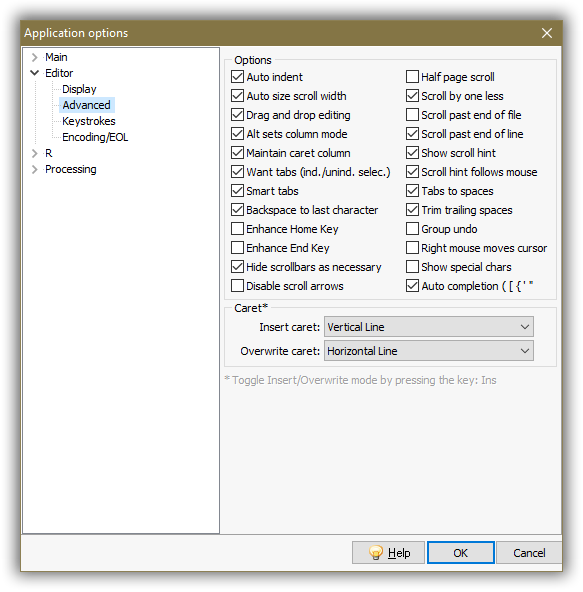
\includegraphics[scale=0.50]{./res/app_editor_advanced.png}~~
  \caption{Editor options: Advanced.}
  \label{fig:editor_advanced}
\end{figure}

\begin{table}
  \begin{footnotesize}
    \begin{tabularx}{\headwidth}{lX}\\
      \hline
      \textbf{Option} & \textbf{Description} \\
      \hline %Options-----
      Auto indent & Will indent the caret (position of the cursor in the current line) on new lines with the same amount of leading white space as the preceding line \\
      Auto size scroll width & Automatically resizes the MaxScrollWidth property when inserting text \\
      Drag and drop editing & Allows you to select a block of text and drag it within the document to another location \\
      Alt sets column mode & Holding down the $<$ALT$>$ key will put the selection mode into column format \\
      Maintain caret column & When moving through lines w/o cursor past EOL, keeps the X position of the cursor \\
      Want tabs (ind./unind. select.) & When tabbing (if there is a selection) $<$TAB$>$ and $<$SHIFT$>$$<$TAB$>$ act as block indent, unindent \\
      Smart tabs & When tabbing, the cursor will go to the next non-white space character of the previous line \\
      Backspace to last character & The cursor will go to the next non-white space character of the line \\
      Enhance home key & Enhances HOME key positioning, similar to visual studio \\
      Enhance end Key & Enhances END key positioning, similar to JDeveloper \\
      Hide scrollbars as necessary & If enabled, then the scrollbars will only show when necessary.
      If you have ScrollPastEOL, then the horizontal bar will always be there (it uses MaxLength instead) \\
      Disable scroll arrows & Disables the scroll bar arrow buttons when you can't scroll in that direction any more \\
      Half page scroll & When scrolling with page-up and page-down commands, only scroll a half page at a time \\
      Scroll by one less & Forces scrolling to be one less \\
      Scroll past end of file & Allows the cursor to go past the end of file marker \\
      Scroll past end of line & Allows the cursor to go past the last character into the white space at the end of a line \\
      Show scroll hint & Shows a hint of the visible line numbers when scrolling vertically \\
      Scroll hint follows mouse & The scroll hint follows the mouse when scrolling vertically \\
      Tabs to spaces & Converts a tab character to a specified number of space characters \\
      Trim trailing spaces & Spaces at the end of lines will be trimmed and not saved \\
      Group undo & When undoing/redoing actions, handle all continuous changes of the same kind in one call instead undoing/redoing
      each command separately \\
      Right mouse moves cursor & When clicking with the right mouse for a pop-up menu, move the cursor to that location \\
      Show special chars & Shows the special characters \\
      \hline %Caret-----
      Insert caret & A list with four options: Vertical line, Horizontal line, Half block and block \\
      Overwrite caret & A list with options: Vertical line, Horizontal line, Half block and block \\
      \hline
    \end{tabularx}
  \end{footnotesize}
  \caption{Display (Options/Editor).}
  \label{tab:editor_advanced}
\end{table}

Figure \ref{fig:editor_advanced} and
Table \ref{tab:editor_advanced}
show the main resources.


\hypertarget{working_editor_encoding_eol}{}
\subsubsection{Encoding/EOL:}
\index{application options!editor encoding}
\index{application options!editor EOL}

\begin{figure}[H]
  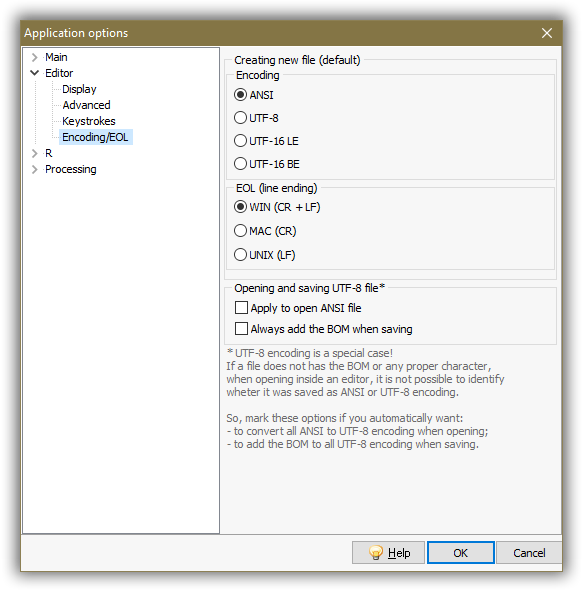
\includegraphics[scale=0.50]{./res/app_editor_encoding.png}\\
  \caption{Editor options: encoding/EOL.}
  \label{fig:editor_encoding}
\end{figure}

This interface
(Figure \ref{fig:editor_encoding})
allows to change the default encoding and EOL when creating new files and
also the user option related to UTF-8 files.


\hypertarget{working_app_r}{}
\subsection{R}
\index{application options!R}

\begin{figure}[h!]
  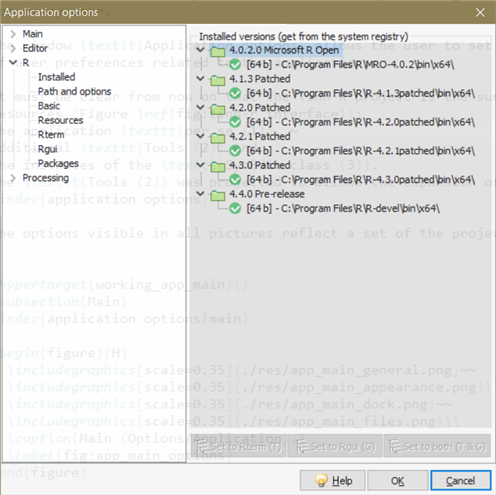
\includegraphics[scale=0.35]{./res/app_r_installed.png}~~
  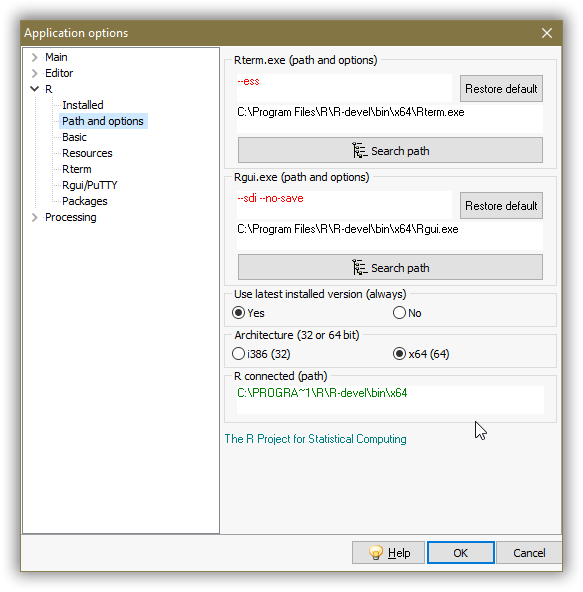
\includegraphics[scale=0.35]{./res/app_r_pathandoptions.png}\\
  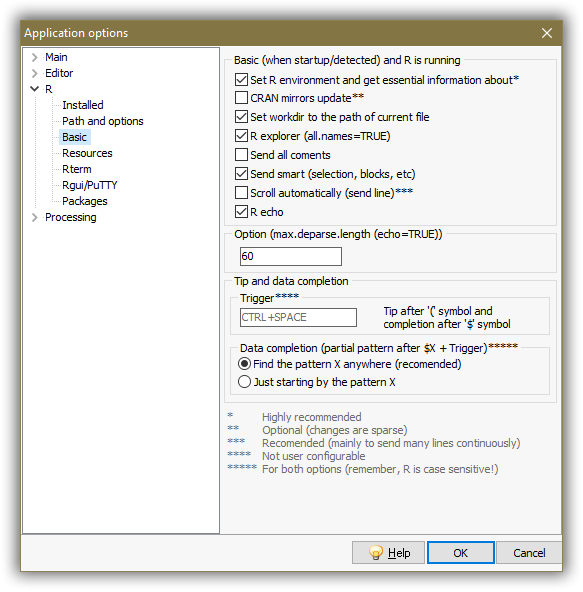
\includegraphics[scale=0.35]{./res/app_r_basic.png}~~
  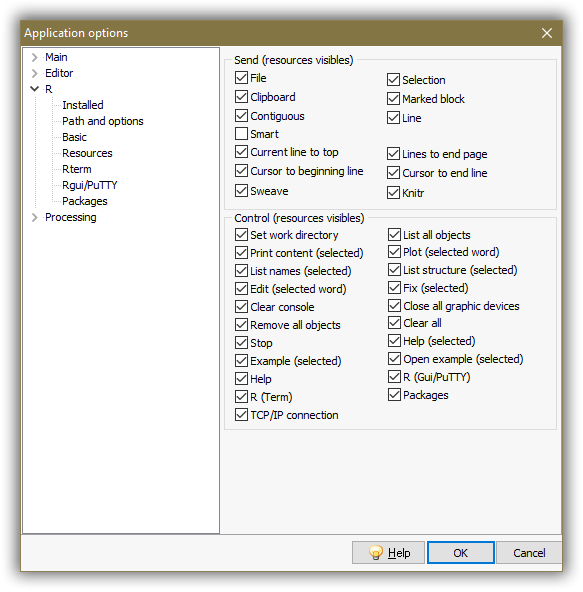
\includegraphics[scale=0.35]{./res/app_r_resources.png}\\
  \caption{R (Options/Application).}
  \label{fig:app_r_a}
\end{figure}

\begin{figure}[h!]
  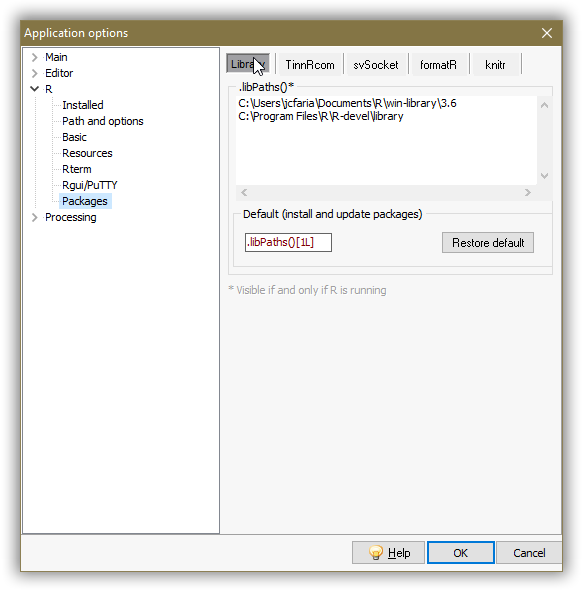
\includegraphics[scale=0.33]{./res/app_r_packages_library.png}~~
  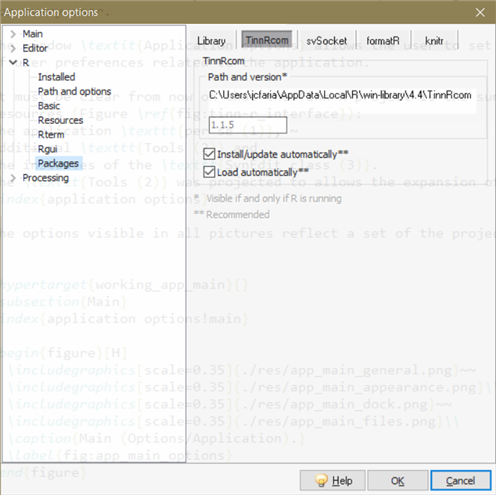
\includegraphics[scale=0.33]{./res/app_r_packages_tinnrcom.png}\\
  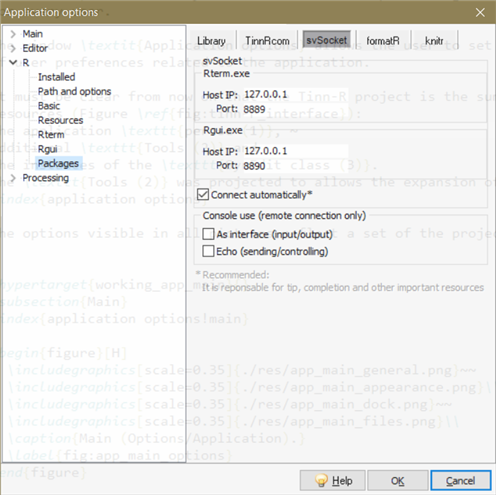
\includegraphics[scale=0.33]{./res/app_r_packages_svsocket.png}\\
  \caption{R (Options/Application).}
  \label{fig:app_r_b}
\end{figure}

\begin{figure}[h!]
  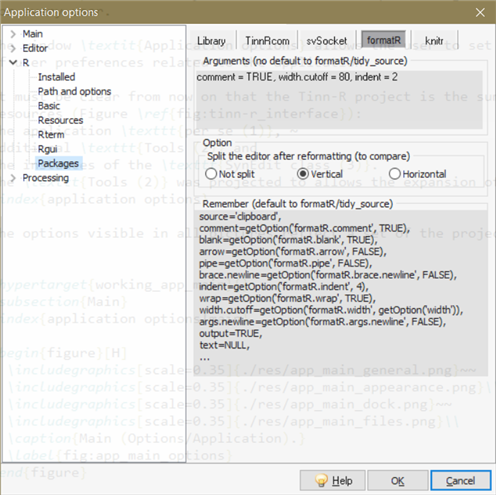
\includegraphics[scale=0.33]{./res/app_r_packages_formatr.png}~~
  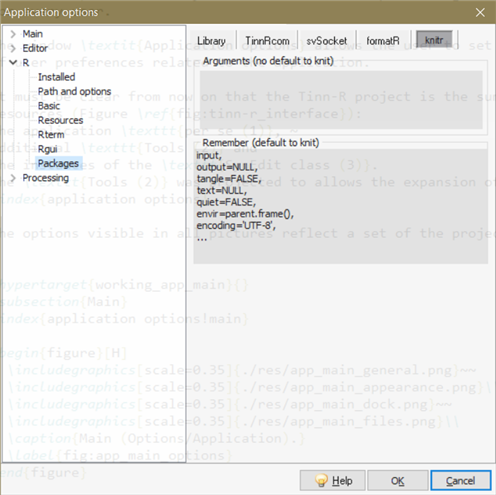
\includegraphics[scale=0.33]{./res/app_r_packages_knitr.png}\\
  \caption{R (Options/Application).}
  \label{fig:app_r_c}
\end{figure}

\begin{figure}[h!]
  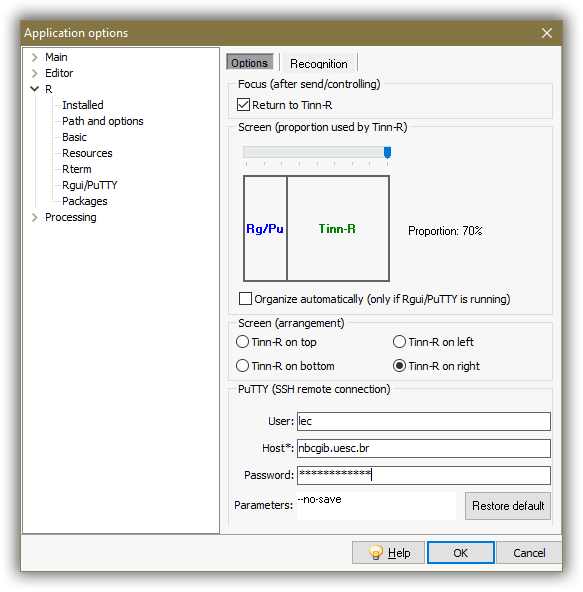
\includegraphics[scale=0.35]{./res/app_r_rgui_options.png}~~
  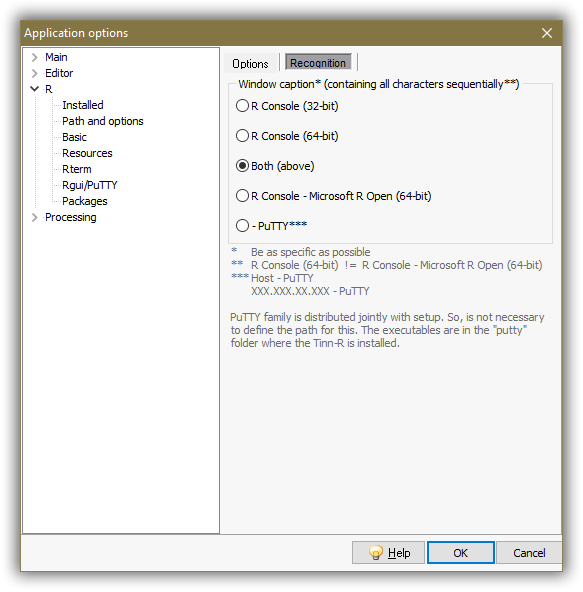
\includegraphics[scale=0.35]{./res/app_r_rgui_recognition.png}\\
  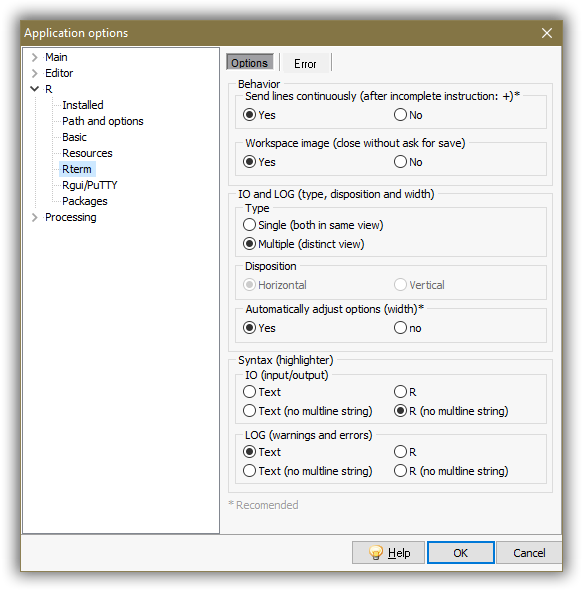
\includegraphics[scale=0.35]{./res/app_r_rterm_options.png}~~
  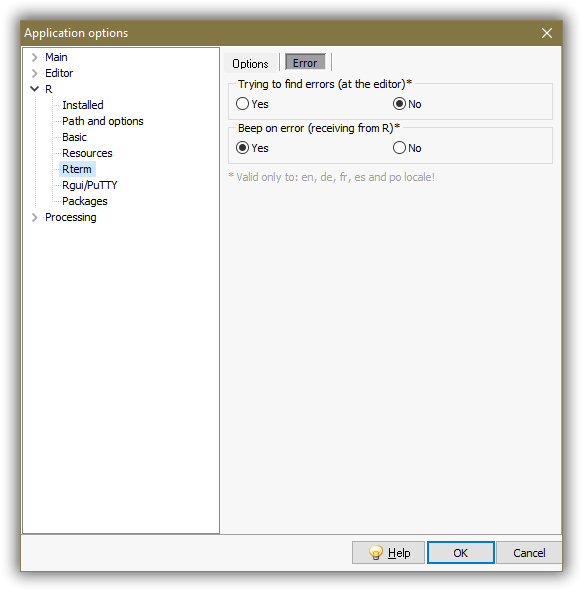
\includegraphics[scale=0.35]{./res/app_r_rterm_error.png}\\
  \caption{R (Options/Application).}
  \label{fig:app_r_d}
\end{figure}

Figures \ref{fig:app_r_a},
        \ref{fig:app_r_b},
        \ref{fig:app_r_c} and
        \ref{fig:app_r_d}
shows a set of options available. As you can see, it allows a high level
of customization with the \RR{} environment.


\hypertarget{working_app_processing}{}
\subsection{Processing}
\index{application options!processing}

\begin{figure}[h!]
  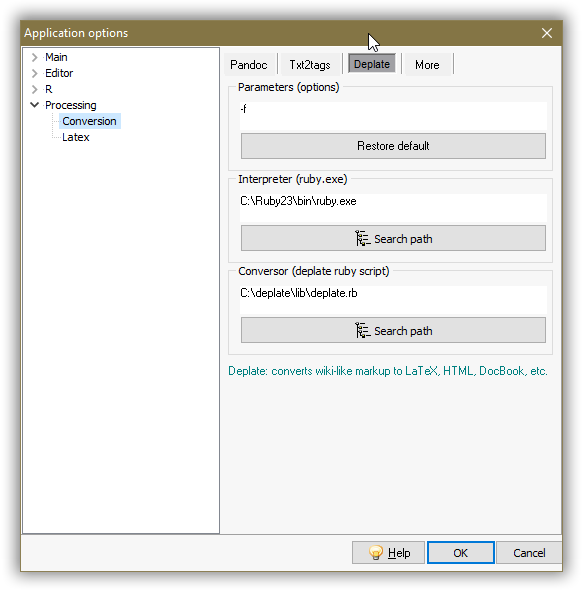
\includegraphics[scale=0.35]{./res/app_processing_conversion_deplate.png}~~
  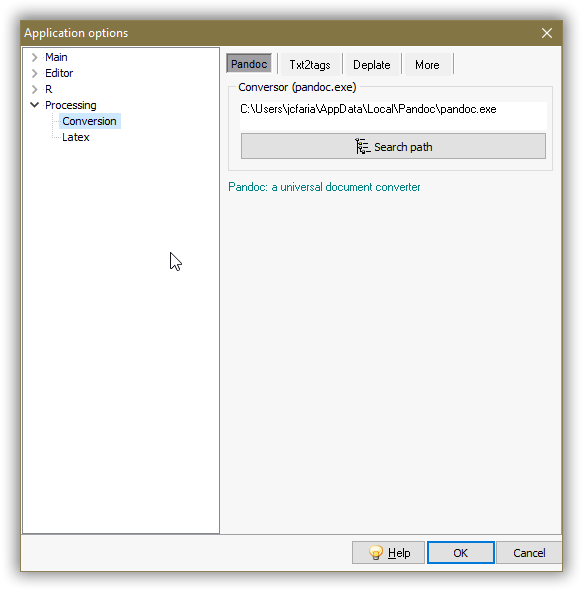
\includegraphics[scale=0.35]{./res/app_processing_conversion_pandoc.png}\\
  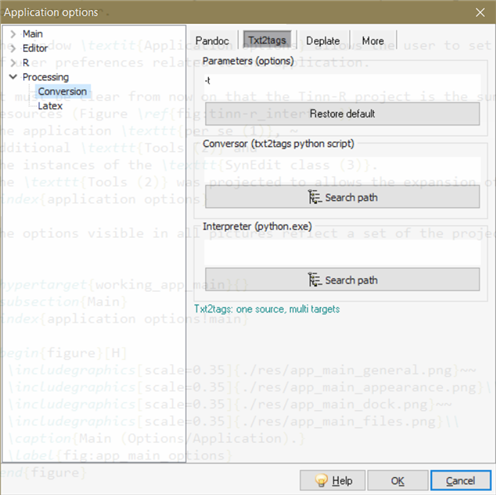
\includegraphics[scale=0.35]{./res/app_processing_conversion_txt2tags.png}~~
  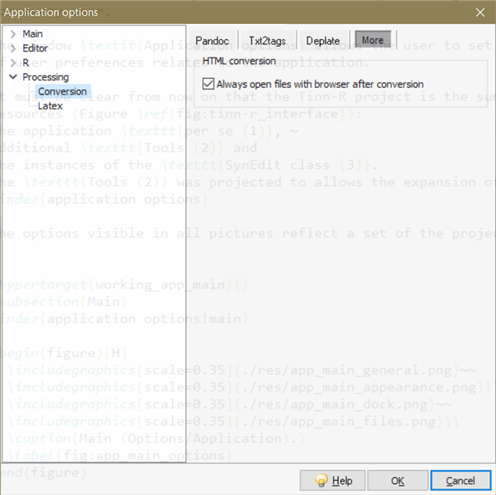
\includegraphics[scale=0.35]{./res/app_processing_conversion_more.png}\\
  \caption{Conversion (Options/Application/Processing).}
  \label{fig:app_processing_conversion_options}
\end{figure}

There are resources
(Figure \ref{fig:app_processing_conversion_options} and
\ref{fig:app_processing_latex_options})
related to conversion (Deplate, Pandoc and Txt2tags) and compilation (Miktex).


\hypertarget{working_app_processing_conversion}{}
\subsubsection{Conversion:}
\index{application options!processing conversion}

Tinn-R project makes it easy to work with these nice conversion tools: Deplate, Pandoc and Txt2tags.
(Figure \ref{fig:app_processing_conversion_options}).


%\newpage
\hypertarget{working_app_processing_latex}{}
\subsubsection{LaTex:}
\index{application options!processing LaTeX}

\begin{figure}[h!]
  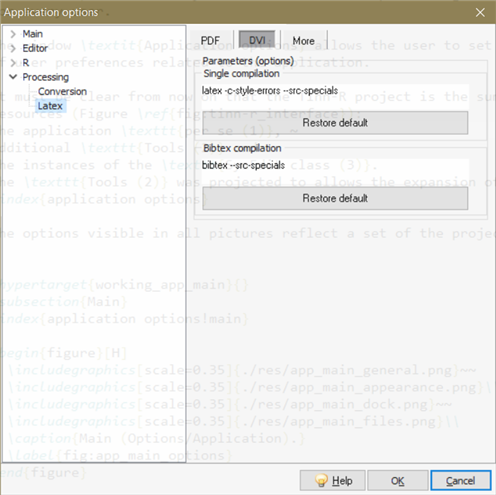
\includegraphics[scale=0.33]{./res/app_processing_latex_dvi.png}~~
  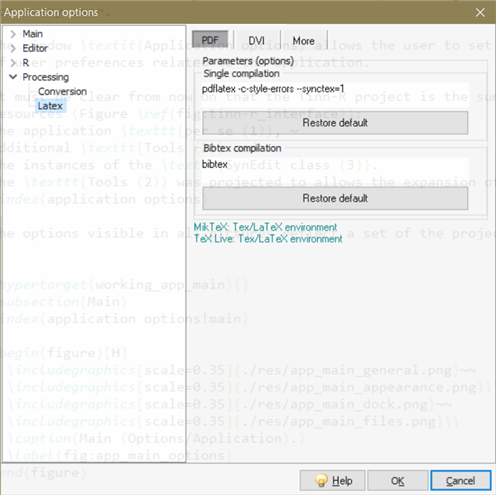
\includegraphics[scale=0.33]{./res/app_processing_latex_pdf.png}\\
  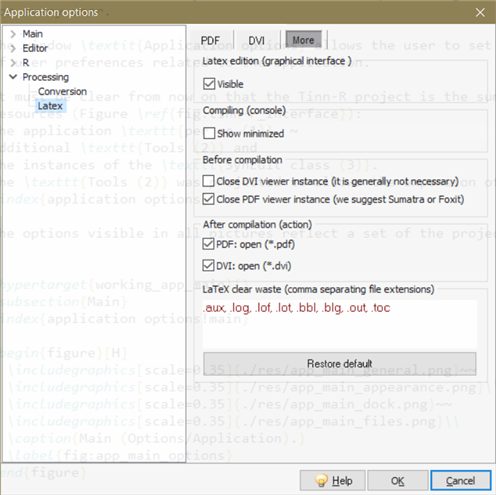
\includegraphics[scale=0.33]{./res/app_processing_latex_more.png}\\
  \caption{Latex (Options/Application/Processing).}
  \label{fig:app_processing_latex_options}
\end{figure}

Tinn-R is not a specific editor to \LaTeX, but it has the basic resources (Figure \ref{fig:app_processing_latex_options}) allowing the user to use the main resources of this environment.
